\section{Результаты}

\subsection{Данные выборки}

\begin{figure}[ht]
	\begin{center}
		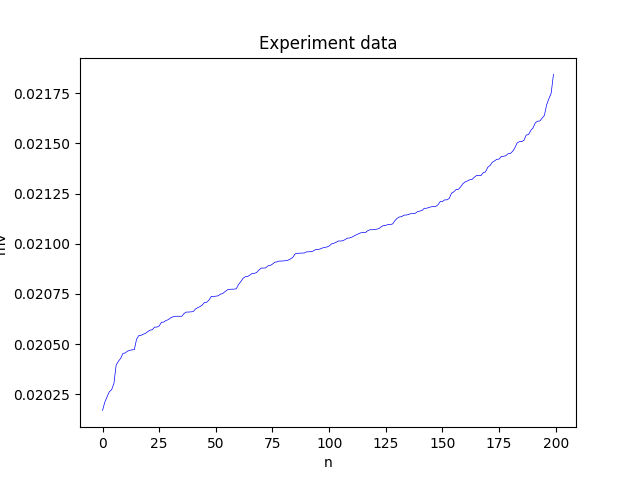
\includegraphics[scale = 0.55]{../images/data.png}
	\end{center}
	\caption{Данные выборки $\bm{X}_1$}
\end{figure}

\begin{figure}[ht]
	\begin{center}
		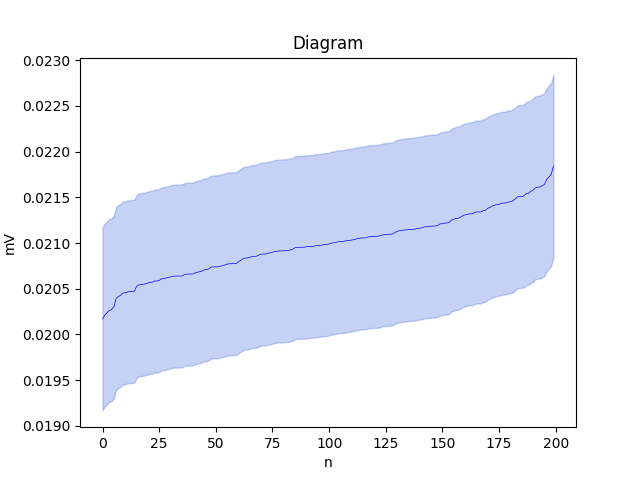
\includegraphics[scale = 0.55]{../images/diagram_beta_None.png}
	\end{center}
	\caption{Диаграмма рассеяния выборки $\bm{X}_1$ с уравновешанным интервалом неопределенности}
\end{figure}

\FloatBarrier

\subsection{Варьирование неопределенности изменений}

При решении задачи линейного программирования \eqref{eq:lin_opt_task}, \eqref{eq:lin_opt_boundaries} были получены следующие результаты: 

\begin{equation*}
	\beta_0 = 0.020, \beta_1 = 6.504 \cdot 10 ^ {-6} 
\end{equation*}

\begin{equation*}
	w_1 = (w^{1}_1, \ldots, w^{n}_1), \sum\limits_{i=1}^{n} w^{i}_1 = 202.831
\end{equation*}

\begin{figure}[ht]
	\begin{center}
		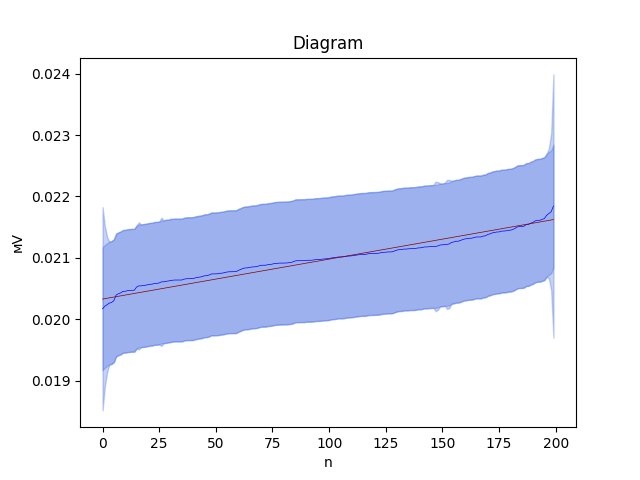
\includegraphics[scale = 0.55]{../images/diagram_and_regress_1.png}
	\end{center}
	\caption{Диаграмма рассеяния выборки $\bm{X}_1$ и регрессионная прямая по модели}
\end{figure}

Красным цветом обозначена регрессионная прямая модели. 

\FloatBarrier

\subsection{Варьирование неопределенности изменений с расширением и сужением интервалов}

При решении задачи линейного программирования \eqref{eq:lin_opt_pos_task}, \eqref{eq:lin_opt_pos_boundaries} были получены следующие результаты: 

\begin{equation*}
	\beta_0 = 0.020, \beta_1 = 5.354 \cdot 10 ^ {-6} 
\end{equation*}

\begin{equation*}
	w_0 = (w^{1}_0, \ldots, w^{n}_0), \sum\limits_{i=1}^{n} w^{i}_0 = 77.636
\end{equation*}

\begin{figure}[ht]
	\begin{center}
		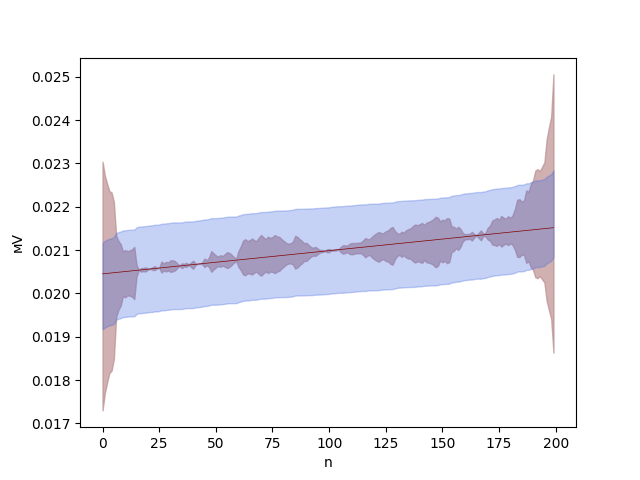
\includegraphics[scale = 0.55]{../images/diagram_and_regress_0.png}
	\end{center}
	\caption{Диаграмма рассеяния выборки $\bm{X}_1$ и регрессионная прямая по модели} \label{pic:lin_opt_pos_task}
\end{figure}

\FloatBarrier

Розовым цветом обозначены скорректированные интервалы выборки $\bm{X}_1$, голубым - первоначальные интервалы. Регрессионная прямая обозначена красным цветом. 

\begin{figure}[ht]
	\begin{center}
		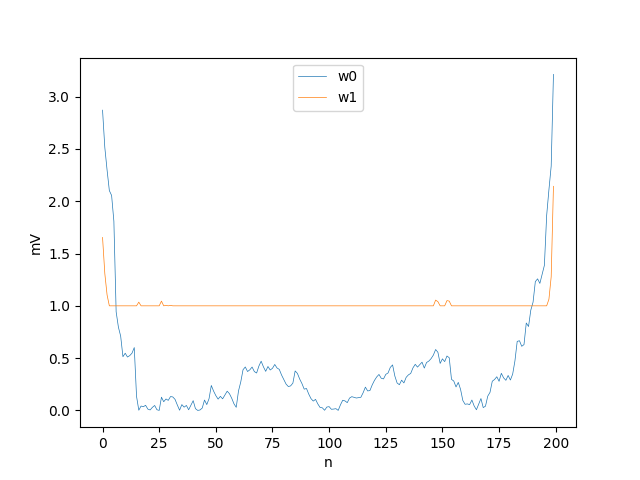
\includegraphics[scale = 0.55]{../images/w0_w1.png}
	\end{center}
	\caption{Векторы $w_0$ и $w_1$} \label{pic:w0_w1}
\end{figure}

\FloatBarrier
\subsection{Анализ регрессионных остатков}

\begin{figure}[ht]
	\begin{center}
		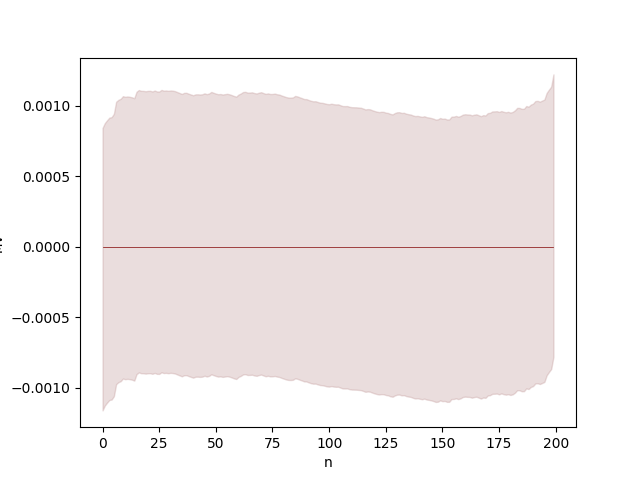
\includegraphics[scale = 0.55]{../images/analysis_of_regression_residuals_1.png}
	\end{center}
	\caption{Диаграмма рассеяния регрессионных остатков для модели без сужения интервалов} \label{pic:without_reduction}
\end{figure}

\begin{figure}[ht]
	\begin{center}
		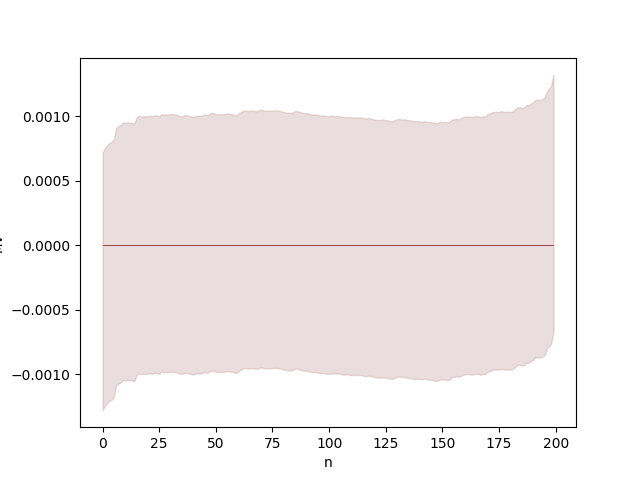
\includegraphics[scale = 0.55]{../images/analysis_of_regression_residuals_0.png}
	\end{center}
	\caption{Диаграмма рассеяния регрессионных остатков для модели с сужением и расширением интервалов} \label{pic:with_reduction}
\end{figure}

\begin{figure}[ht]
	\begin{center}
		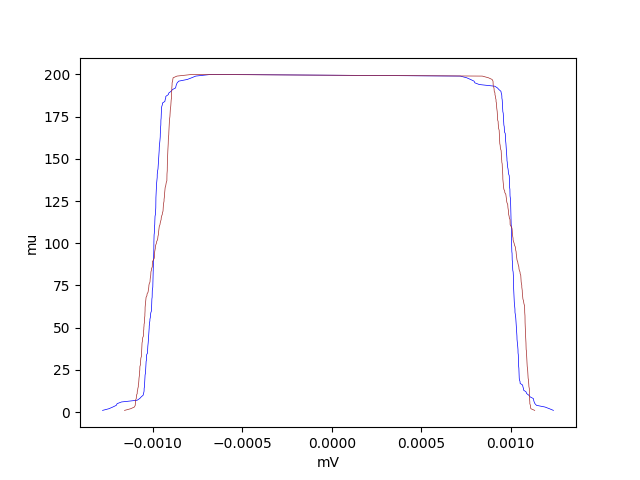
\includegraphics[scale = 0.55]{../images/mu.png}
	\end{center}
	\caption{Частоты элементарных подинтервалов регрессионных остатков при вычислении моды для двух моделей} \label{pic:freq}
\end{figure} 

\FloatBarrier

\textbf{Красный график} -- график частот элементарных подинтервалов регрессионных остатков при вычислении моды модели без сужения интервалов. \\
\textbf{Синий график} -- график частот элементарных подинтервалов регрессионных остатков при вычислении моды модели с сужением и расширением интервалов. \\

Меры совместности регрессионных остатков: \\

\begin{tabular}{c c}
	mode $\bm{X}^0 = [-0.0007, 0.0007]$ & $\bm{J}_i(\bm{X}^0) = 0.5335$ \\
	mode $\bm{X}^1 = [-0.0008, 0.0008]$ & $\bm{J}_i(\bm{X}^1) = 0.6808$ \\
\end{tabular}

Здесь $\bm{X}^{0}, \bm{X}^{1}$ -- регрессионные остатки выборки $\bm{X}_1$, вычисленные с использованием разных условий оптимизации. \\

\FloatBarrier
\subsection{Информационное множество задачи} 


\begin{figure}[ht]
	\begin{center}
		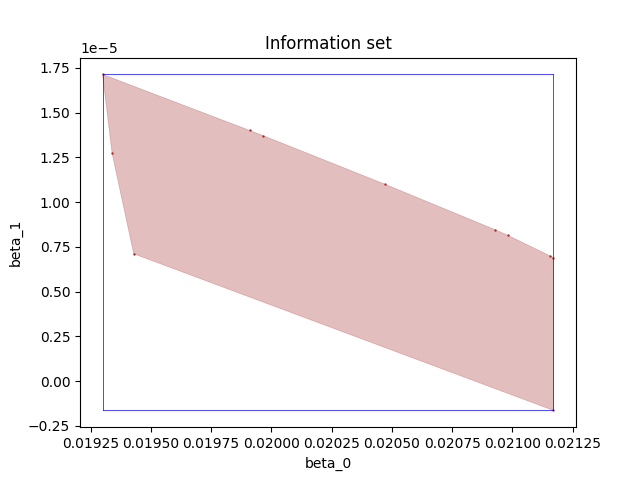
\includegraphics[scale = 0.55]{../images/inform_set.png}
	\end{center}
	\caption{Информационное множество задачи по заданной модели -- красный брус, интервальная оболочка -- синий брус}
\end{figure}

\FloatBarrier
\subsection{Коридор совместных зависимостей}

Внешние интервальные оценки параметров модели: 

\begin{equation*}
	\text{mid} \beta_0 = [0.0193, 0.0212]
\end{equation*}

\begin{equation*}
	\text{mid} \beta_1 = [-1.6382e-06, 1.7129e-05]
\end{equation*}

Подставляя эти значения в уравнение регрессии, получаем:

\begin{equation}
	\bm{x}(k) = \text{mid} \beta_0 + \text{mid} \beta_1 \cdot k
\end{equation}

\begin{figure}[ht]
	\begin{center}
		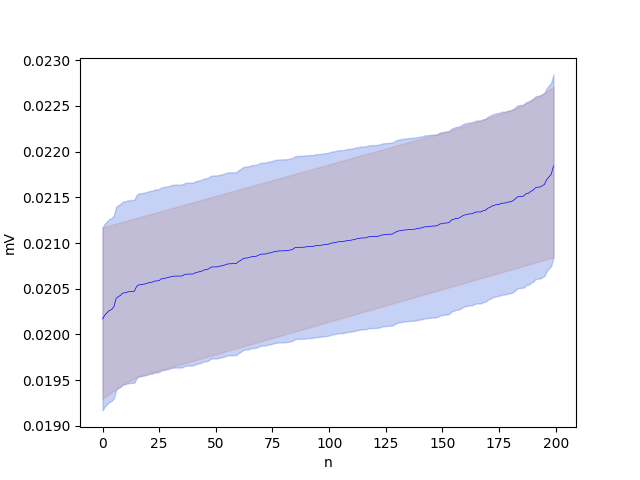
\includegraphics[scale = 0.55]{../images/corridor_of_joint_dependencies.png}
	\end{center}
	\caption{Коридор совместных зависимостей}
\end{figure}

\FloatBarrier

\subsection{Прогноз вне области данных}

\begin{figure}[ht]
	\begin{center}
		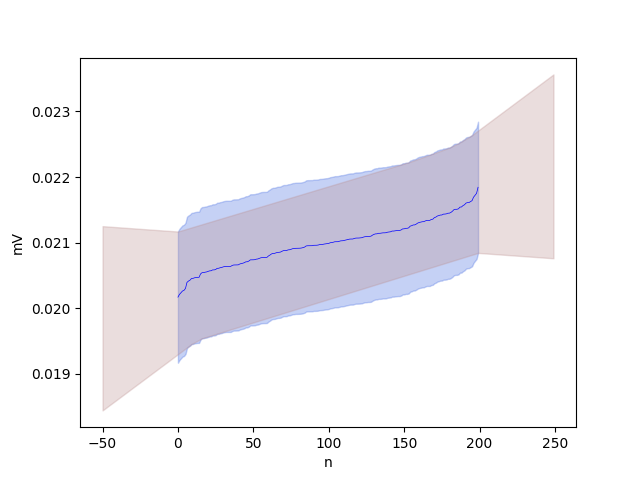
\includegraphics[scale = 0.55]{../images/corridor_of_joint_dependencies_prediction.png}
	\end{center}
	\caption{Коридор совместных зависимостей. Построение прогноза}
\end{figure}


\newpage
